\section{Results}\label{sec:results}

We organize our findings around six experiments. E1 establishes the core comparison of all seven operators on \mnist; E2 and E3 isolate \emph{how much} and \emph{where} we sample; E4 shows that Monte Carlo averaging recovers most of the single-sample cost; E5 probes input-noise robustness; and E6 confirms the picture on the harder \cifar\ task, where the categorical analogue collapses outright. Throughout, ``cost'' means the single-sample accuracy drop relative to \detmode, and we read the gradient-variance column as the mechanistic driver of that cost.

\subsection{E1: Core comparison on \mnist}\label{sec:e1}

\tabref{tab:e1} reports all seven operators on a 3-layer MLP (3 seeds, sampling placed after hidden-1). We measure single-sample accuracy, MC-10 accuracy (averaging 10 stochastic passes), \nll, \ece, the train$-$test generalization gap, and the per-step gradient variance at the sampling layer.

\begin{table}[t]
\centering
\caption{\textbf{E1: core comparison on \mnist}\ (MLP, 3 seeds, sampling after hidden-1). Acc (1 sample) and Acc (MC-10) are test accuracies; Gen-gap is train$-$test accuracy; Grad-var is the gradient variance at the sampling layer. Best value per column in \textbf{bold}. The cost ordering \gaussreparam$\approx$\detmode\ $\ll$ \bernoullist\ $\ll$ categorical (\gumbelsoft, \gumbelst) is tracked exactly by the Grad-var column.}
\label{tab:e1}
\resizebox{\textwidth}{!}{%
\begin{tabular}{lcccccc}
\toprule
Mode & Acc (1 sample) & Acc (MC-10) & \nll & \ece & Gen-gap & Grad-var \\
\midrule
\detmode & \textbf{0.9776} & 0.9776 & 0.088 & 0.0118 & 0.0172 & $0$ \\
\dropout & 0.9655 & 0.9781 & 0.123 & 0.0115 & 0.0118 & $9.3\times10^{-7}$ \\
\gaussnoise & 0.9800 & \textbf{0.9804} & 0.091 & 0.0123 & 0.0152 & $5.3\times10^{-8}$ \\
\gaussreparam & 0.9773 & 0.9775 & 0.089 & 0.0098 & 0.0111 & $1.5\times10^{-6}$ \\
\bernoullist & 0.9499 & 0.9663 & 0.166 & \textbf{0.0070} & 0.0109 & $8.0\times10^{-8}$ \\
\gumbelsoft & 0.8995 & 0.9191 & 0.386 & 0.0194 & 0.0006 & $7.1\times10^{-6}$ \\
\gumbelst & 0.8735 & 0.8859 & 0.511 & 0.0150 & $-0.0214$ & $1.5\times10^{-5}$ \\
\bottomrule
\end{tabular}%
}
\end{table}

\begin{figure}[t]
\centering
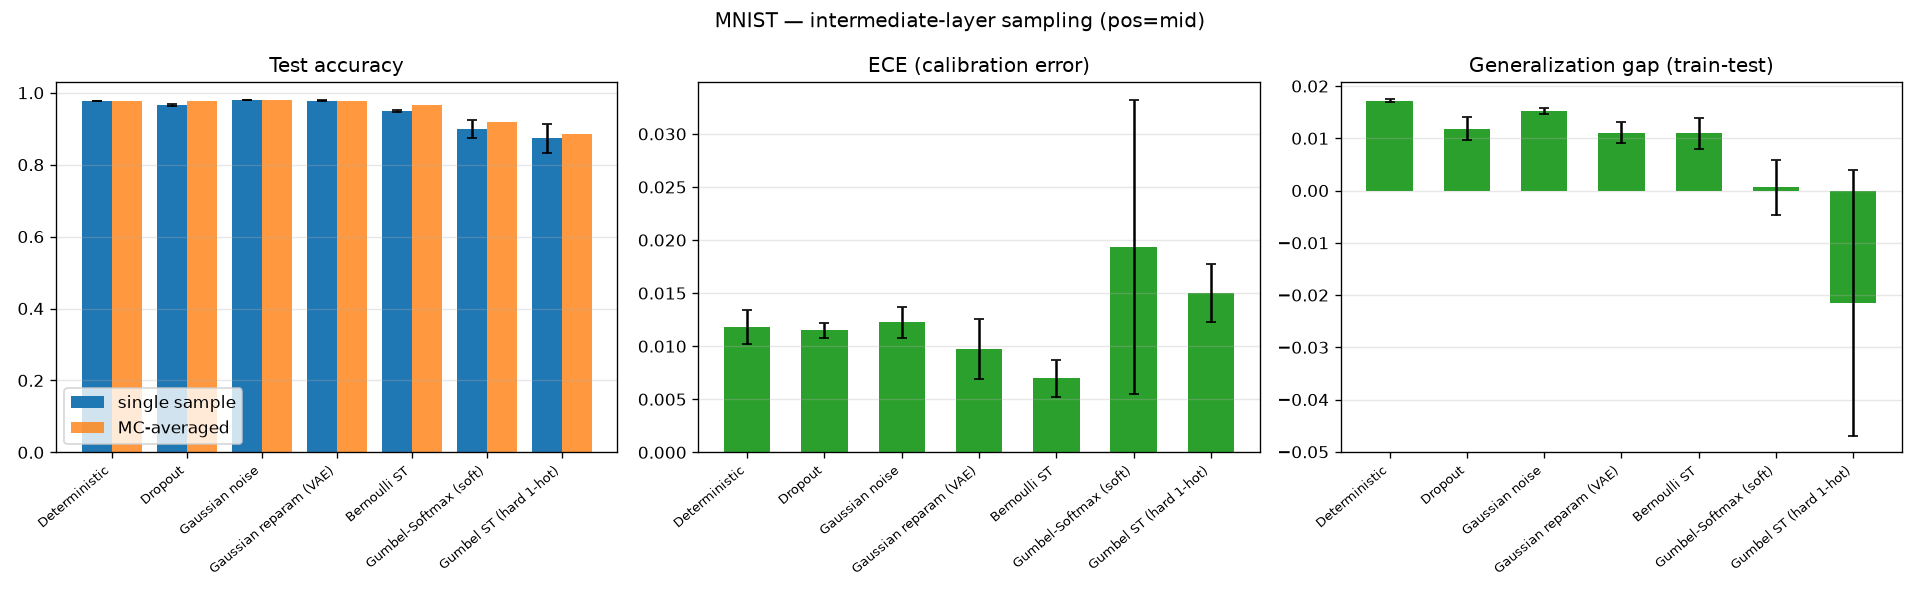
\includegraphics[width=0.8\linewidth]{figures/E1_core_mnist_bars.png}
\caption{\textbf{E1 on \mnist.} Single-sample test accuracy for the seven activation operators (MLP, 3 seeds, sampling after hidden-1). Continuous variants (\gaussnoise, \gaussreparam) sit at the deterministic reference line; \bernoullist\ pays a small cost; the categorical softmax analogues (\gumbelsoft, \gumbelst) are by far the most expensive.}
\label{fig:e1}
\end{figure}

Paired $t$-tests against \detmode\ on single-sample accuracy confirm the ordering: \bernoullist\ $\Delta=-2.77$ pts ($p=0.0015$), \gumbelsoft\ $\Delta=-7.82$ pts ($p=0.031$), and \gumbelst\ $\Delta=-10.4$ pts ($p=0.048$) are all significant losses. \gaussreparam\ is statistically indistinguishable from deterministic ($\Delta=-0.03$ pts, $p=0.83$ --- effectively free), and \gaussnoise\ is a small, non-significant gain ($\Delta=+0.24$ pts, $p=0.11$). \figref{fig:e1} shows the same picture visually.

\para{Reading.} Three patterns stand out. First, the cost ordering is Gaussian $\approx 0 \ll$ Bernoulli $\ll$ categorical: replacing deterministic activations with continuous reparameterized samples costs essentially nothing, while a hard one-hot categorical sample costs over ten accuracy points. Second, gentle stochasticity \emph{improves} calibration --- \ece\ drops to $0.0070$ for \bernoullist\ and $0.0098$ for \gaussreparam\ versus $0.0118$ for \detmode\ --- and the generalization gap shrinks for \emph{every} sampling variant (from $0.0172$ down to as little as $0.0006$, even going negative for \gumbelst). Sampling is acting as a regularizer. Third, and most telling, the Grad-var column ranks the operators in the same order as their accuracy cost. The categorical operators inject the most gradient variance ($7.1\times10^{-6}$ and $1.5\times10^{-5}$) and pay the most; the reparameterized continuous operators inject little and pay nothing. Gradient variance is the mechanism.

\subsection{E2: How much you sample (temperature / noise)}\label{sec:e2}

E2 isolates the \emph{intensity} of sampling. For \gumbelsoft\ we sweep the temperature $\tau$; for \gaussnoise\ we sweep the noise scale $\sigma$ (\tabref{tab:e2}, \figref{fig:e2}).

\begin{table}[t]
\centering
\caption{\textbf{E2: how much you sample.} Left: \gumbelsoft\ test accuracy as a function of temperature $\tau$. Right: \gaussnoise\ test accuracy as a function of noise scale $\sigma$. Sharper categorical sampling (low $\tau$) is more aggressive and far more costly; Gaussian noise is gentle across two decades of $\sigma$.}
\label{tab:e2}
\begin{tabular}{cc@{\hspace{3em}}cc}
\toprule
\multicolumn{2}{c}{\gumbelsoft} & \multicolumn{2}{c}{\gaussnoise} \\
\cmidrule(r){1-2}\cmidrule(l){3-4}
$\tau$ & Acc & $\sigma$ & Acc \\
\midrule
0.1 & 0.664 & 0.1 & 0.979 \\
0.5 & 0.900 & 0.3 & 0.980 \\
1.0 & 0.957 & 0.6 & 0.980 \\
2.0 & 0.969 & 1.0 & 0.978 \\
5.0 & 0.976 & 2.0 & 0.976 \\
\bottomrule
\end{tabular}
\end{table}

\begin{figure}[t]
\centering
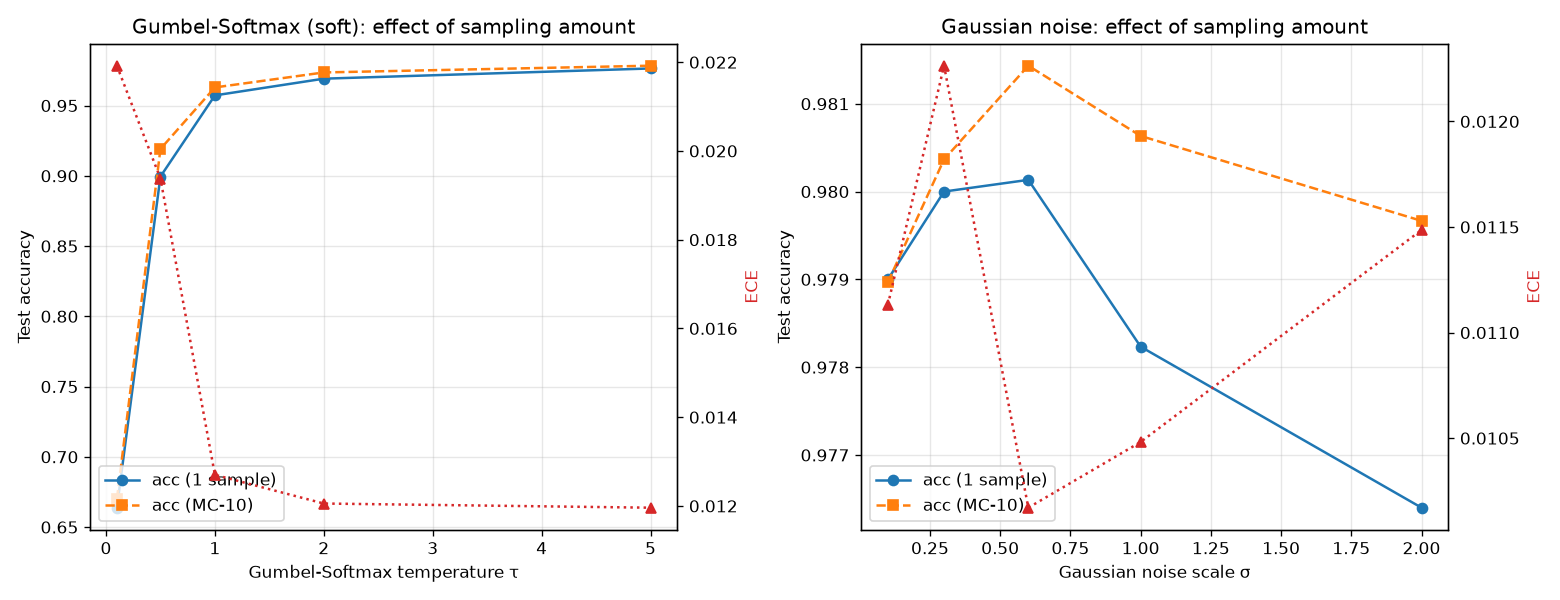
\includegraphics[width=0.8\linewidth]{figures/E2_sweep.png}
\caption{\textbf{E2 sweeps.} \gumbelsoft\ accuracy rises monotonically as temperature $\tau$ increases (sampling fades), while \gaussnoise\ accuracy is essentially flat across $\sigma$, with a mild robustness sweet-spot near $\sigma\approx0.3$--$0.6$.}
\label{fig:e2}
\end{figure}

\para{Reading.} The two sweeps tell opposite stories. For the categorical operator, lower $\tau$ means a sharper softmax, a more aggressive (more nearly one-hot) sample, and a larger cost: accuracy climbs monotonically from $66.4\%$ at $\tau=0.1$ to $97.6\%$ at $\tau=5.0$. As $\tau$ grows the softmax flattens toward uniform and the act of sampling effectively fades, so accuracy approaches the deterministic level. This cleanly separates the \emph{distributional layer} from the \emph{act of sampling}: the cost lives in the sampling, not in having a distribution. The Gaussian operator, by contrast, is gentle across two decades of $\sigma$ (all within $0.976$--$0.980$), with only a mild robustness sweet-spot around $\sigma\approx0.3$--$0.6$.

\subsection{E3: Where you sample (layer position)}\label{sec:e3}

E3 moves the \samplinglayer\ between two positions: pos$=0$ (after hidden-1) and pos$=1$ (after hidden-2, nearer the output). \tabref{tab:e3} reports three representative operators.

\begin{table}[t]
\centering
\caption{\textbf{E3: where you sample.} Single-sample test accuracy with the \samplinglayer\ after hidden-1 (pos$=0$) versus after hidden-2 (pos$=1$, nearer the output). Sampling closer to the output is consistently cheaper.}
\label{tab:e3}
\begin{tabular}{lcc}
\toprule
Mode & pos$=0$ (after hidden-1) & pos$=1$ (after hidden-2) \\
\midrule
\bernoullist & 0.9499 & 0.9783 \\
\gaussreparam & 0.9773 & 0.9795 \\
\gumbelst & 0.8735 & 0.8886 \\
\bottomrule
\end{tabular}
\end{table}

\para{Reading.} Sampling closer to the output is consistently cheaper for every operator. \bernoullist\ recovers almost the full deterministic accuracy when moved to pos$=1$ ($0.9499\to0.9783$), and even \gumbelst\ improves ($0.8735\to0.8886$). Two factors compound: fewer remaining layers are disrupted by the injected noise, and for the categorical operators the one-active-unit bottleneck sits nearer the already-low-dimensional decision, where collapsing to a sparse representation does less damage.

\subsection{E4: MC-averaging recovers the cost}\label{sec:e4}

E4 averages $K$ stochastic forward passes at inference and sweeps $K\in\{1,5,20,50\}$ (\tabref{tab:e4}, \figref{fig:e4}).

\begin{table}[t]
\centering
\caption{\textbf{E4: MC-averaging.} Test accuracy as a function of the number of averaged stochastic passes $K$. Averaging recovers most of the single-sample cost for high-variance operators; the low-variance \gaussreparam\ has almost nothing to recover.}
\label{tab:e4}
\begin{tabular}{lcccc}
\toprule
Mode & $K{=}1$ & $K{=}5$ & $K{=}20$ & $K{=}50$ \\
\midrule
\dropout & 0.9655 & 0.9766 & 0.9793 & 0.9795 \\
\gumbelsoft & 0.8995 & 0.9174 & 0.9209 & 0.9220 \\
\gaussreparam & 0.9773 & 0.9774 & 0.9774 & 0.9774 \\
\bottomrule
\end{tabular}
\end{table}

\begin{figure}[t]
\centering
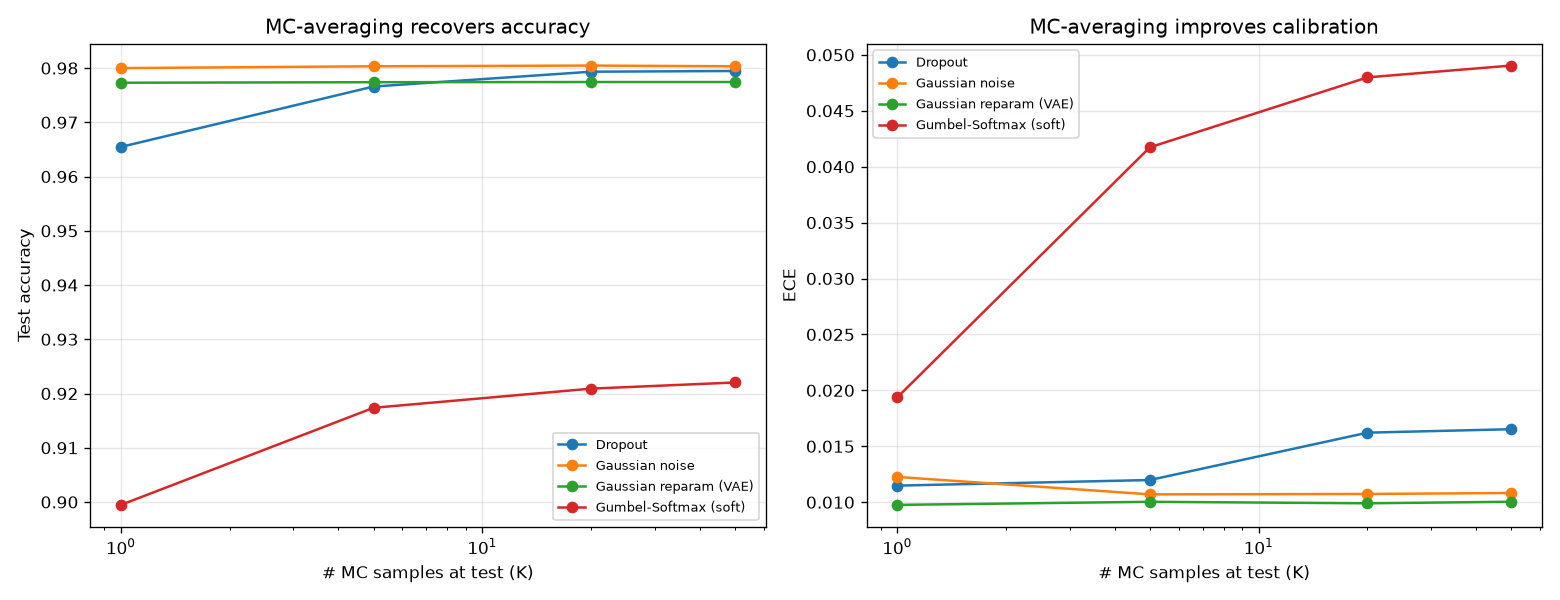
\includegraphics[width=0.8\linewidth]{figures/E4_mc.png}
\caption{\textbf{E4: MC-averaging recovers the cost.} Accuracy versus number of averaged passes $K$. High-variance operators (\dropout, \gumbelsoft) climb sharply with $K$ as the average approaches the expectation over the activation distribution; \gaussreparam\ is flat because its single-sample estimate is already near-deterministic.}
\label{fig:e4}
\end{figure}

\para{Reading.} Averaging many stochastic passes approximates the expectation over the activation distribution --- exactly as averaging softmax samples approximates the class distribution --- and recovers most of the single-sample loss: \dropout\ gains $+1.4$ pts ($0.9655\to0.9795$) and \gumbelsoft\ gains $+2.3$ pts ($0.8995\to0.9220$). The low-variance \gaussreparam\ is flat (all $\approx0.9774$): its single sample is already so close to the expectation that there is almost nothing to recover. One caveat: MC-averaging \emph{categorical} samples can \emph{raise} \ece, because averaging near-one-hot draws yields overconfident mean probabilities --- so the accuracy recovery does not come free on calibration.

\subsection{E5: Robustness to input Gaussian noise (\mnist)}\label{sec:e5}

E5 corrupts test inputs with additive Gaussian noise of scale $\sigma\in\{0.0,0.5,1.0,1.5\}$ (\tabref{tab:e5}, \figref{fig:e5}).

\begin{table}[t]
\centering
\caption{\textbf{E5: robustness to input Gaussian noise (\mnist).} Test accuracy at increasing input corruption $\sigma$. \dropout\ (MC-10) is best at every corrupted severity (\textbf{bold}); continuous \gaussreparam\ tracks \detmode; categorical \gumbelst\ starts lower but degrades relatively gracefully.}
\label{tab:e5}
\begin{tabular}{lcccc}
\toprule
Mode & $\sigma{=}0.0$ & $\sigma{=}0.5$ & $\sigma{=}1.0$ & $\sigma{=}1.5$ \\
\midrule
\detmode & 0.9776 & 0.9719 & 0.9421 & 0.8769 \\
\dropout (MC-10) & 0.9782 & 0.9733 & \textbf{0.9514} & \textbf{0.8988} \\
\gaussreparam & 0.9775 & 0.9704 & 0.9397 & 0.8733 \\
\gumbelst & 0.8854 & 0.8782 & 0.8501 & 0.7984 \\
\bottomrule
\end{tabular}
\end{table}

\begin{figure}[t]
\centering
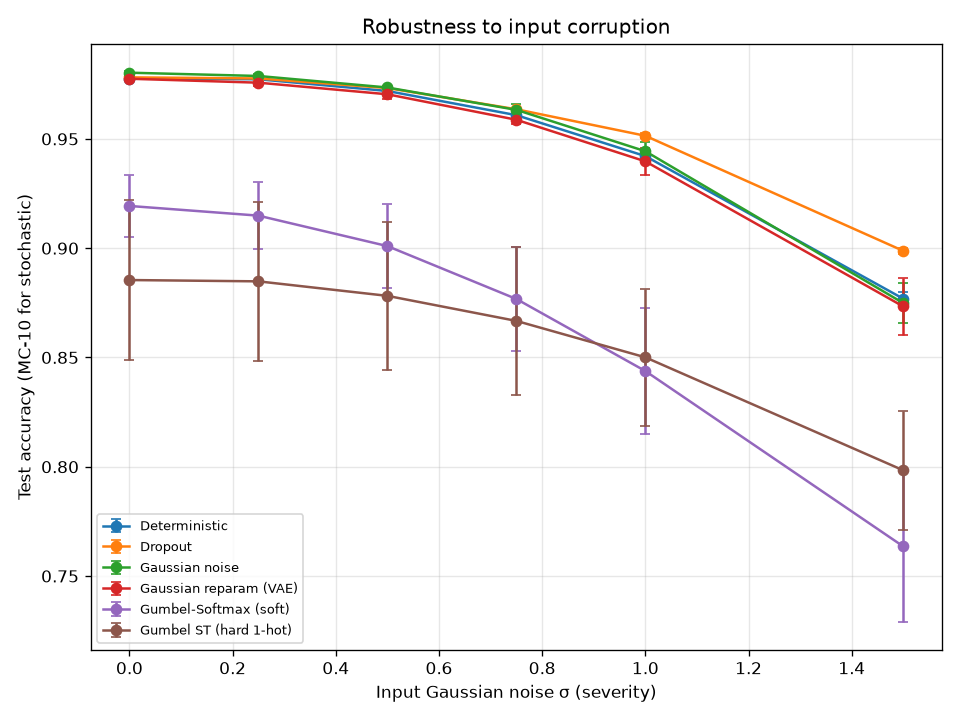
\includegraphics[width=0.8\linewidth]{figures/E5_robust.png}
\caption{\textbf{E5: input-noise robustness on \mnist.} Accuracy versus input corruption scale $\sigma$. \dropout\ with MC-10 averaging is most robust at every severity; \gaussreparam\ tracks \detmode\ closely; \gumbelst\ starts lower but its curve degrades at a comparable rate.}
\label{fig:e5}
\end{figure}

\para{Reading.} The robustness benefit is real but modest, and it is driven mainly by \dropout\ with MC-averaging rather than by intermediate-layer sampling per se. \dropout\ (MC-10) is best at every corrupted severity, with $+1$ pt at $\sigma=1.0$ ($0.9514$ vs $0.9421$) and $+2.2$ pts at $\sigma=1.5$ ($0.8988$ vs $0.8769$). Continuous \gaussreparam\ simply tracks \detmode, offering no robustness edge, while categorical \gumbelst\ starts much lower but degrades relatively gracefully. Overall, hypothesis H5 (that activation sampling buys robustness) is only weakly supported.

\subsection{E6: \cifar\ confirmation (the striking result)}\label{sec:e6}

E6 repeats the core comparison on \cifar\ with a small CNN (3 seeds), where the harder task widens the divide between operator families (\tabref{tab:e6}, \figref{fig:e6}).

\begin{table}[t]
\centering
\caption{\textbf{E6: \cifar\ confirmation}\ (small CNN, 3 seeds). On the harder task, continuous \gaussreparam\ matches/beats deterministic accuracy while sharply improving \nll\ and \ece, and \bernoullist\ gives the best calibration and smallest gap --- but the literal categorical softmax analogues collapse toward chance. Best per column in \textbf{bold}.}
\label{tab:e6}
\resizebox{\textwidth}{!}{%
\begin{tabular}{lccccc}
\toprule
Mode & Acc (1 sample) & Acc (MC-10) & \nll & \ece & Gen-gap \\
\midrule
\detmode & 0.7503 & 0.7503 & 0.941 & 0.1119 & 0.2253 \\
\dropout & 0.7298 & 0.7645 & 0.962 & 0.0987 & 0.1845 \\
\gaussnoise & 0.7456 & 0.7472 & 0.939 & 0.1240 & 0.2288 \\
\gaussreparam & \textbf{0.7548} & \textbf{0.7553} & \textbf{0.784} & 0.0741 & 0.2084 \\
\bernoullist & 0.7384 & 0.7650 & 0.833 & \textbf{0.0681} & \textbf{0.1458} \\
\gumbelsoft & 0.1000 & 0.1000 & 2.316 & 0.030 & $-0.000$ \\
\gumbelst & 0.2555 & 0.2574 & 1.895 & 0.038 & 0.001 \\
\bottomrule
\end{tabular}%
}
\end{table}

\begin{figure}[t]
\centering
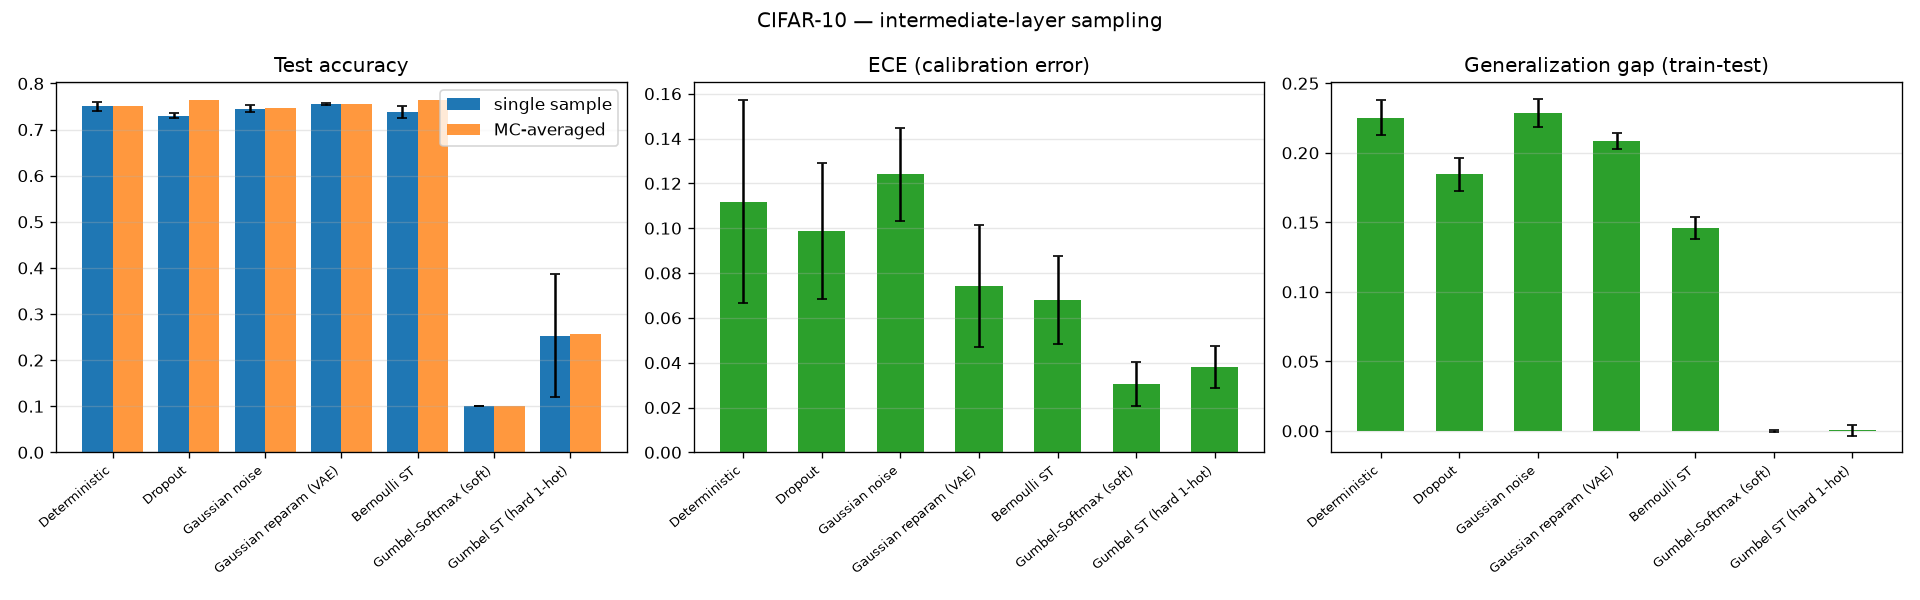
\includegraphics[width=0.8\linewidth]{figures/E6_core_cifar10_bars.png}
\caption{\textbf{E6 on \cifar.} Single-sample test accuracy (small CNN, 3 seeds). Continuous \gaussreparam\ matches or beats the deterministic reference, while the categorical softmax analogues \gumbelsoft\ and \gumbelst\ collapse toward chance ($10\%$ and $25\%$): forcing all CNN features through a single sampled unit is too severe a bottleneck to optimize.}
\label{fig:e6}
\end{figure}

\para{Reading.} On the harder task the divide widens. Continuous \gaussreparam\ matches and slightly beats deterministic accuracy ($75.5\%$ vs $75.0\%$) while cutting \nll\ from $0.94$ to $0.78$ and \ece\ from $0.112$ to $0.074$ --- continuous sampling is again essentially free, and here it is the best-calibrated high-accuracy model. \bernoullist\ gives the best calibration of all ($\ece=0.068$) and the smallest generalization gap ($0.146$ vs $0.225$ deterministic), confirming its regularizing effect. But the literal categorical softmax analogues \emph{collapse}: \gumbelsoft\ falls to chance ($10\%$) and the hard one-hot \gumbelst\ reaches only $25\%$. Forcing all CNN features through a single sampled unit is too severe a bottleneck --- and too high in gradient variance --- to optimize. This is a concrete instance of the VQ-VAE \citep{oord2017vqvae} caution about collapsed hidden samples: the operation that is benign on the final softmax becomes catastrophic when applied to a wide intermediate layer of a convolutional feature extractor.
